\documentclass[12pt,a4paper]{article}
\usepackage[utf8]{inputenc}
\usepackage[polish]{babel}
\usepackage[T1]{fontenc}
\usepackage{amsmath}
\usepackage{amsfonts}
\usepackage{amssymb}
\usepackage{graphicx}
\usepackage{float}
\usepackage{hyperref}
\usepackage{geometry}
\usepackage{booktabs}
\usepackage{subcaption}

\geometry{margin=2.5cm}

\title{Laboratorium 2 - Interpretowalność modeli ML}
\author{Mateusz Łopaciński}
\date{\today}

\begin{document}

\maketitle

\section{Wprowadzenie}

W ramach laboratorium przeprowadzono analizę interpretowalności modeli ML z wykorzystaniem metody LIME. Eksperymenty obejmowały analizę danych tabularnych (zbiór Adult) oraz obrazów z wykorzystaniem różnych sieci neuronowych.

\section{Analiza tabularna - LIME}

\subsection{Porównanie modeli}

Wykorzystano MLPClassifier (3 warstwy: 200-100-50 neuronów, ReLU, Adam) zamiast XGBoost z tutorialu. MLP osiągnął dokładność 81.48\%.

\subsection{Analiza trzech przykładów z tutorialu}

\subsubsection{Przykład 1653}

Oba modele poprawnie przewidziały >50K. XGBoost silnie podkreślał Capital Gain jako główny czynnik, podczas gdy MLP rozłożył wagę między Capital Gain, Capital Loss (ujemny) i fnlwgt (ujemny).

\begin{figure}[H]
  \centering
  \begin{subfigure}{0.45\textwidth}
    \centering
    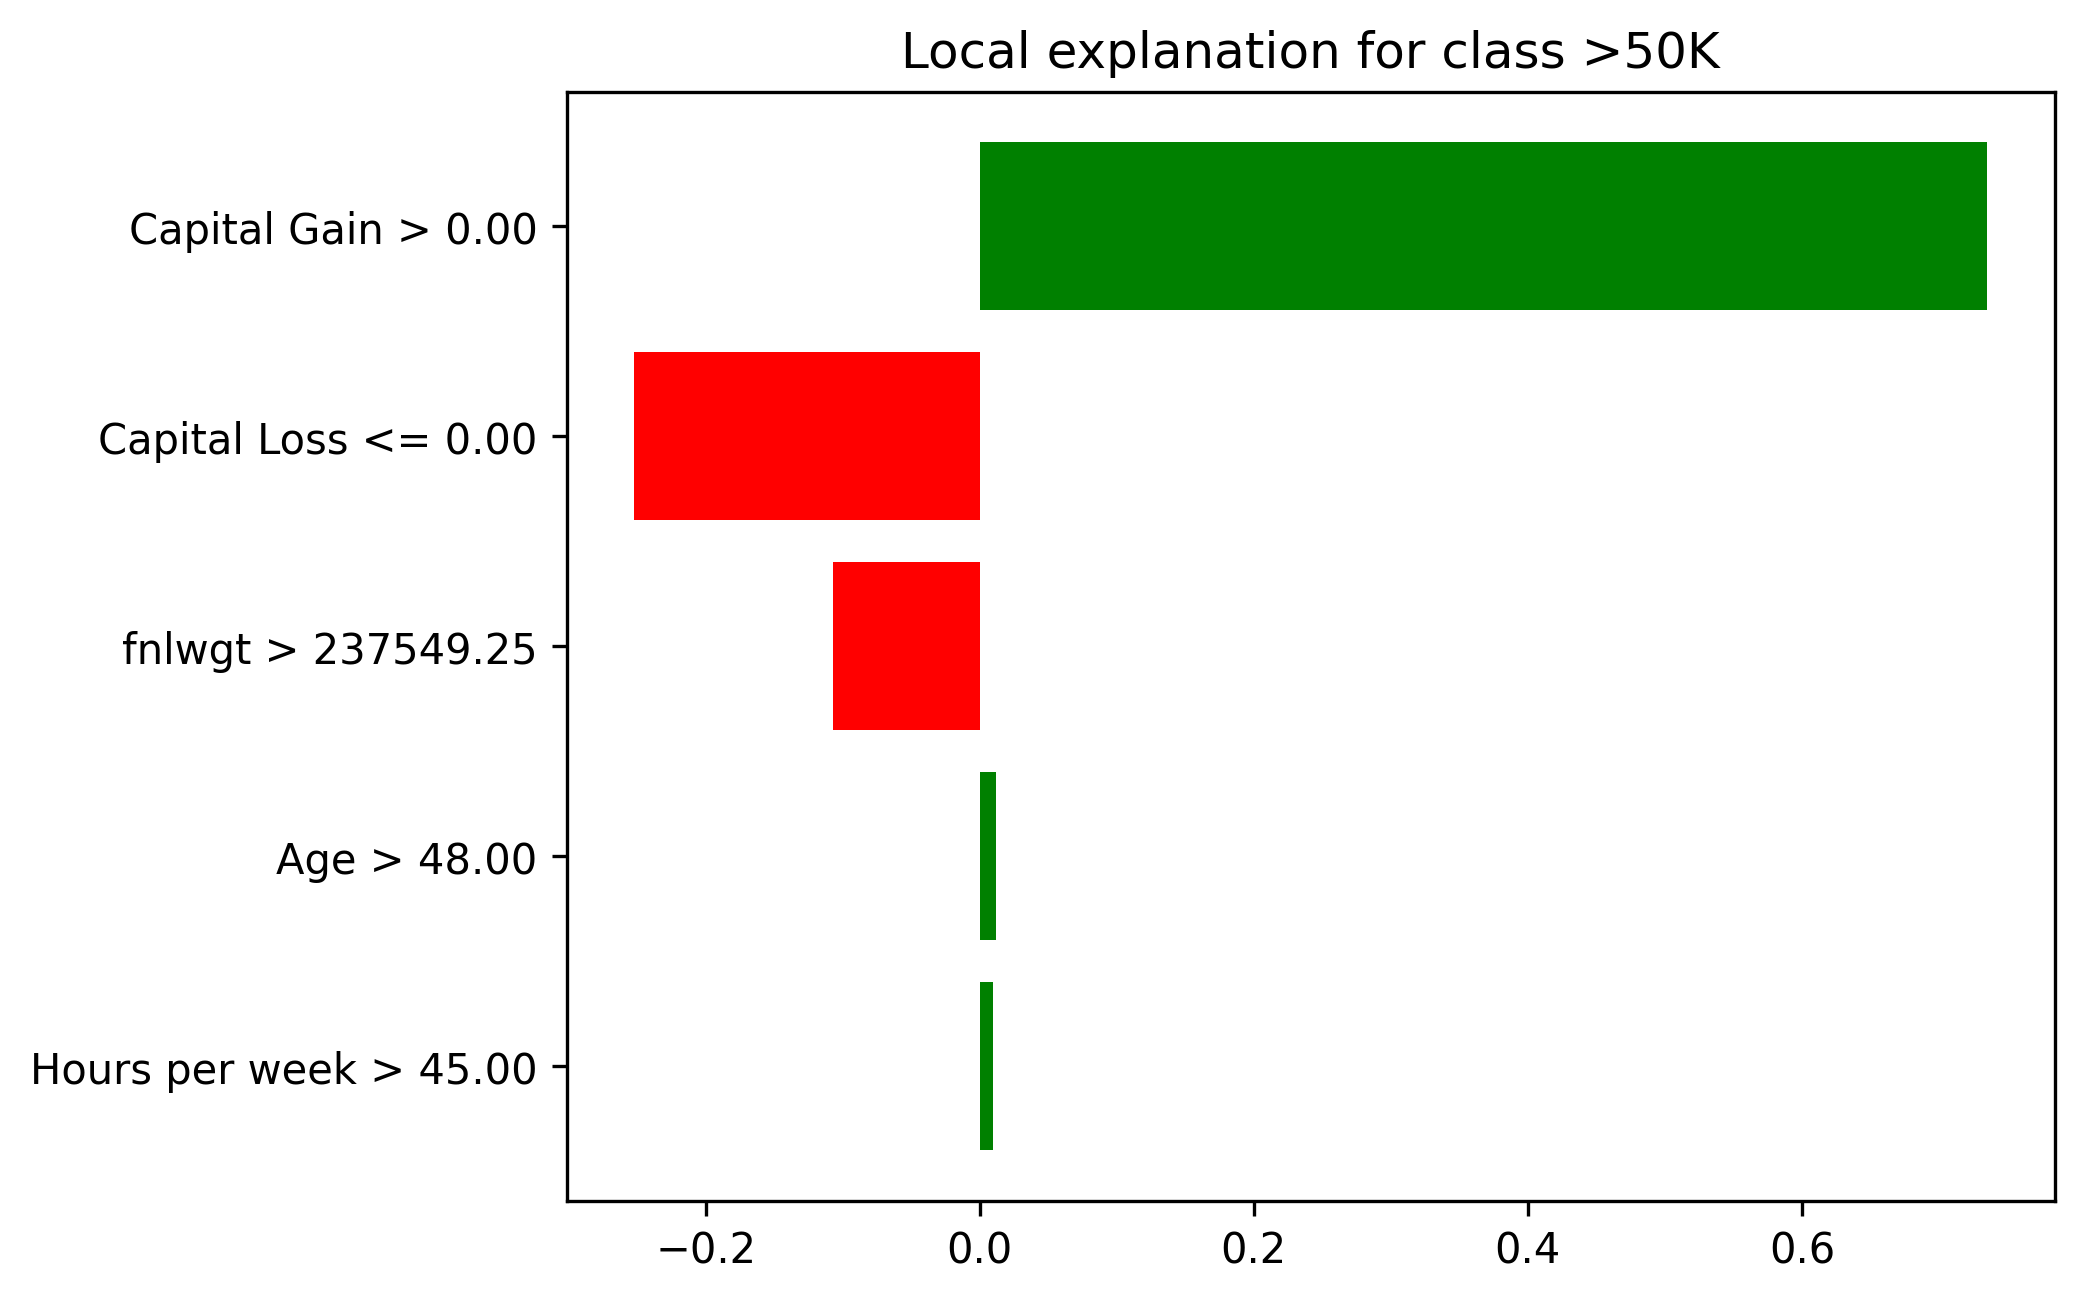
\includegraphics[width=\textwidth]{../out/mlp-1653.png}
    \caption{MLPClassifier}
  \end{subfigure}
  \begin{subfigure}{0.45\textwidth}
    \centering
    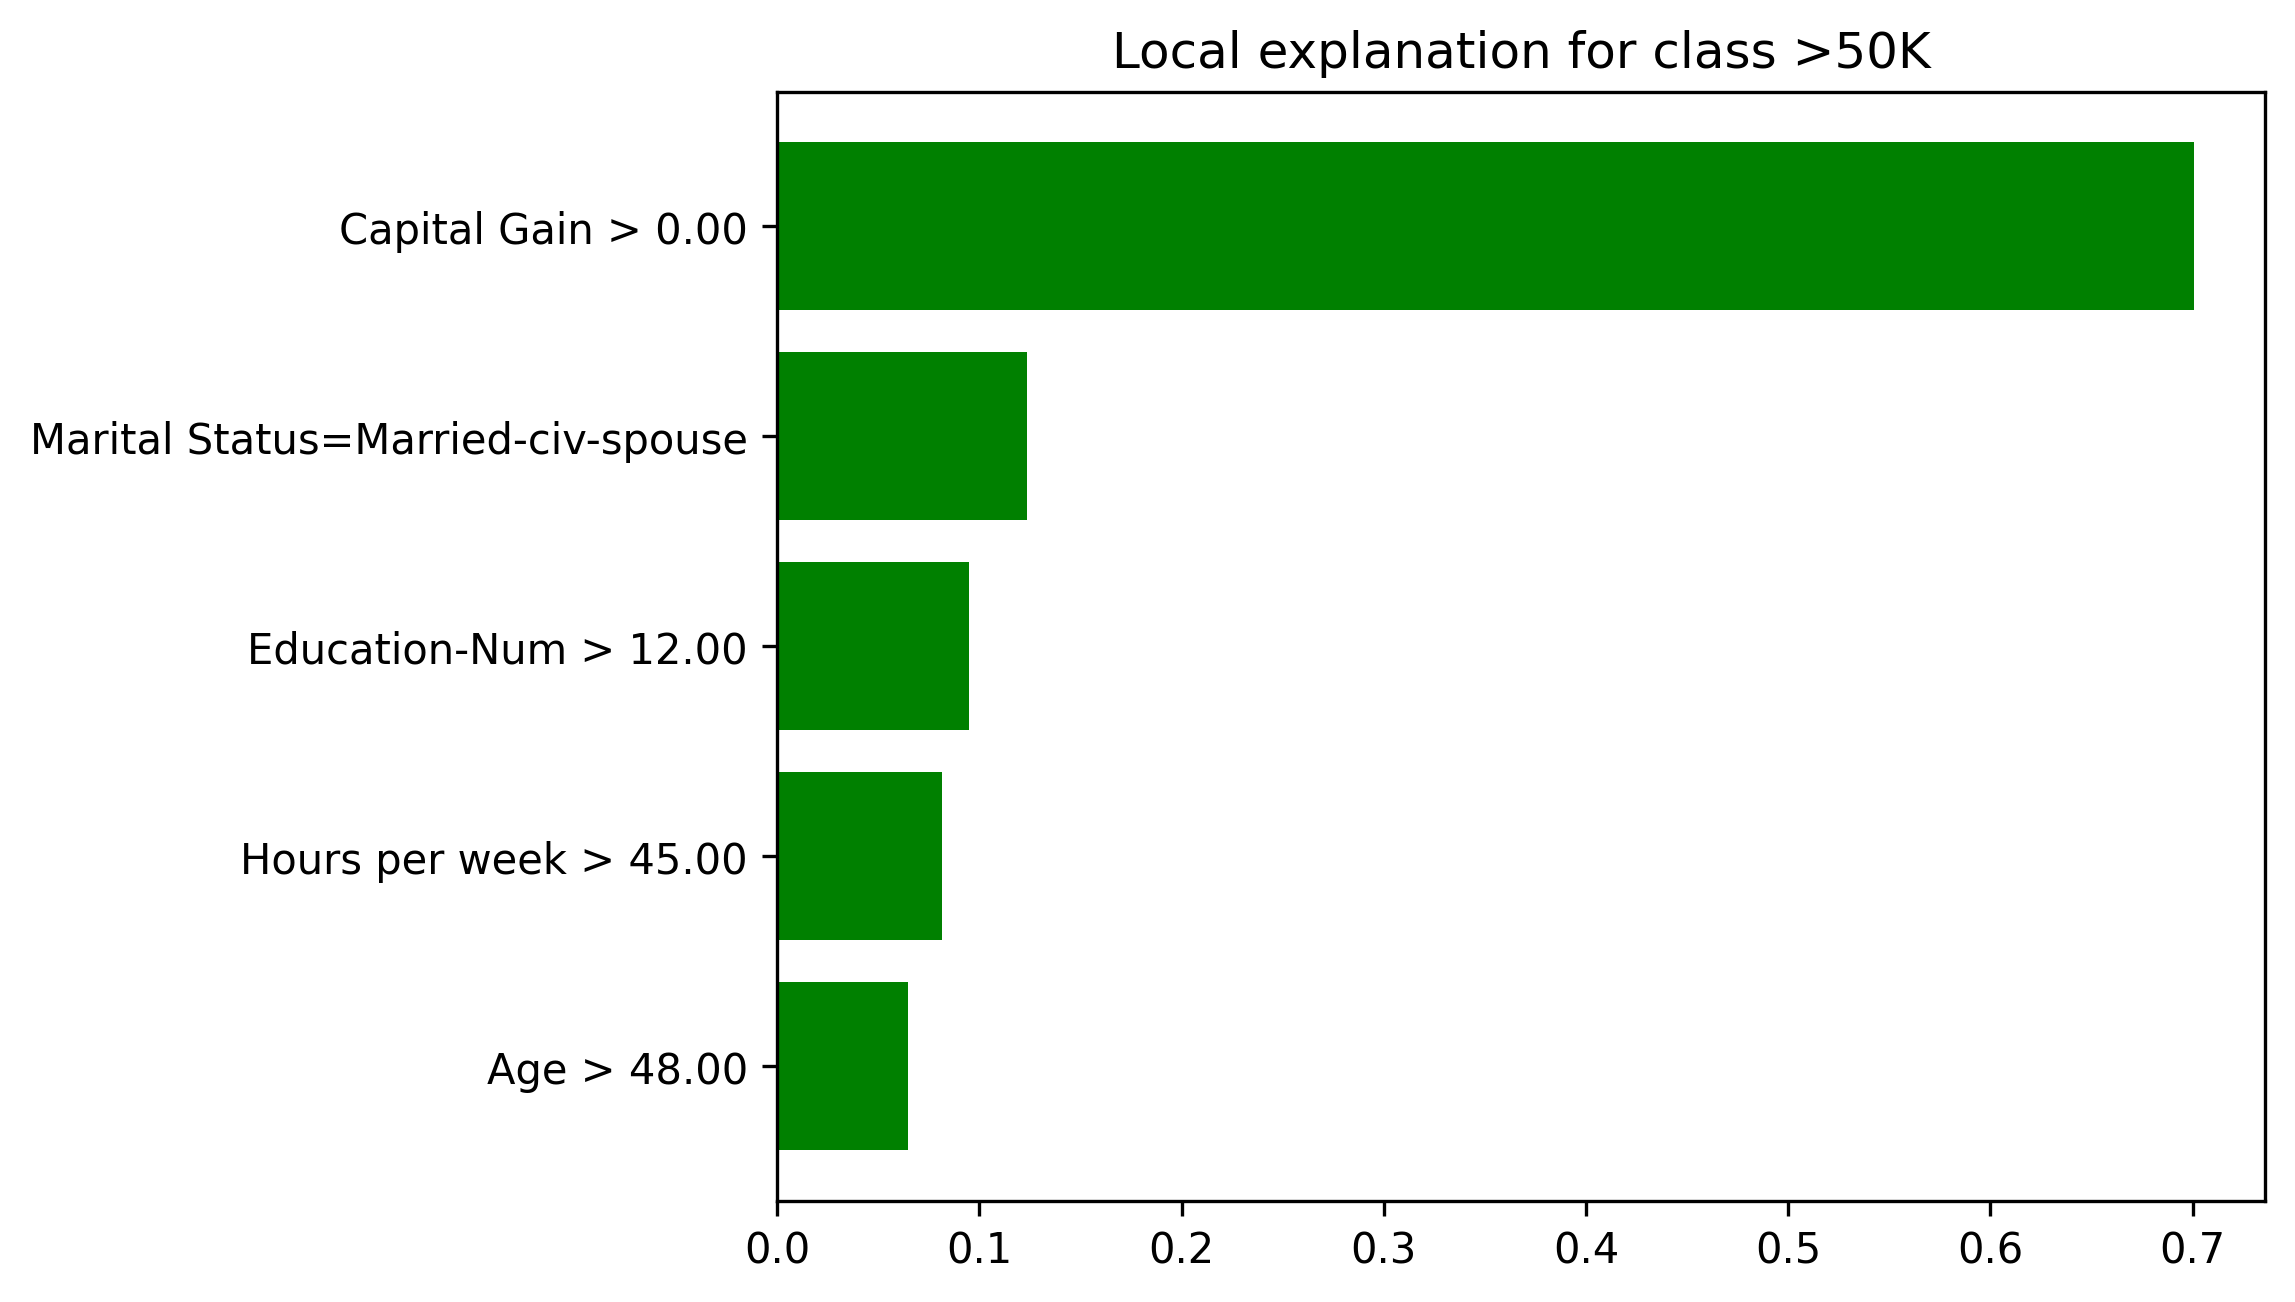
\includegraphics[width=\textwidth]{../out/xgboost-1653.png}
    \caption{XGBoost}
  \end{subfigure}
  \caption{Wyjaśnienia LIME dla przykładu 1653}
\end{figure}

\subsubsection{Przykład 92}

Oba modele poprawnie przewidziały <=50K. Oba interpretowały brak Capital Gain jako silny negatywny czynnik, ale różniły się wagi dla Marital Status i Hours per week.

\begin{figure}[H]
  \centering
  \begin{subfigure}{0.45\textwidth}
    \centering
    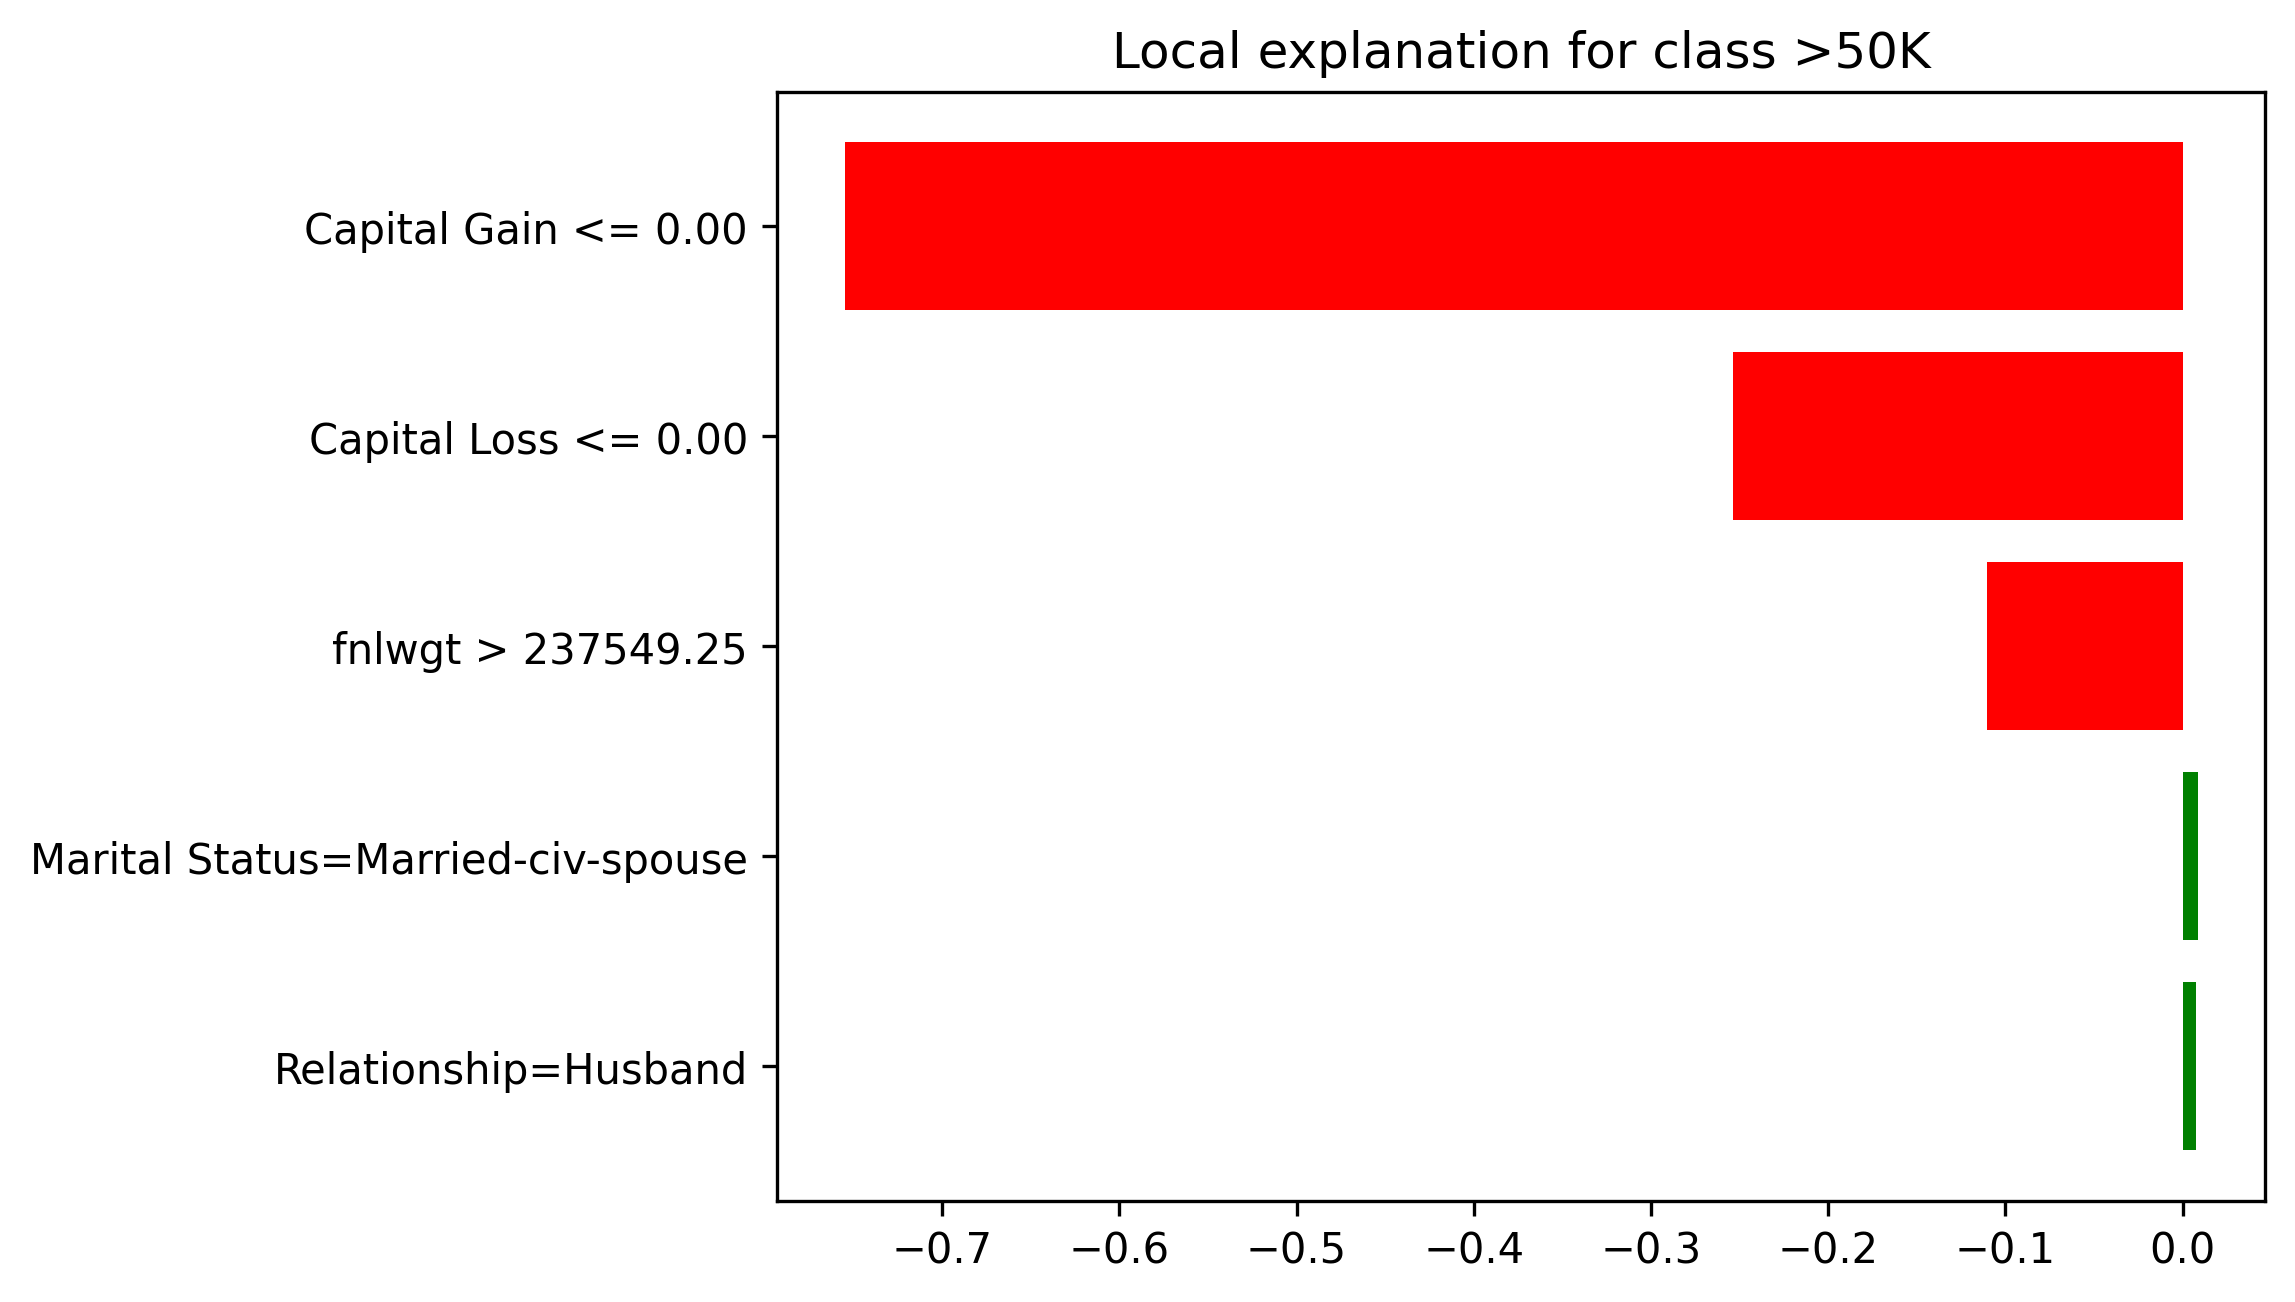
\includegraphics[width=\textwidth]{../out/mlp-92.png}
    \caption{MLPClassifier}
  \end{subfigure}
  \begin{subfigure}{0.45\textwidth}
    \centering
    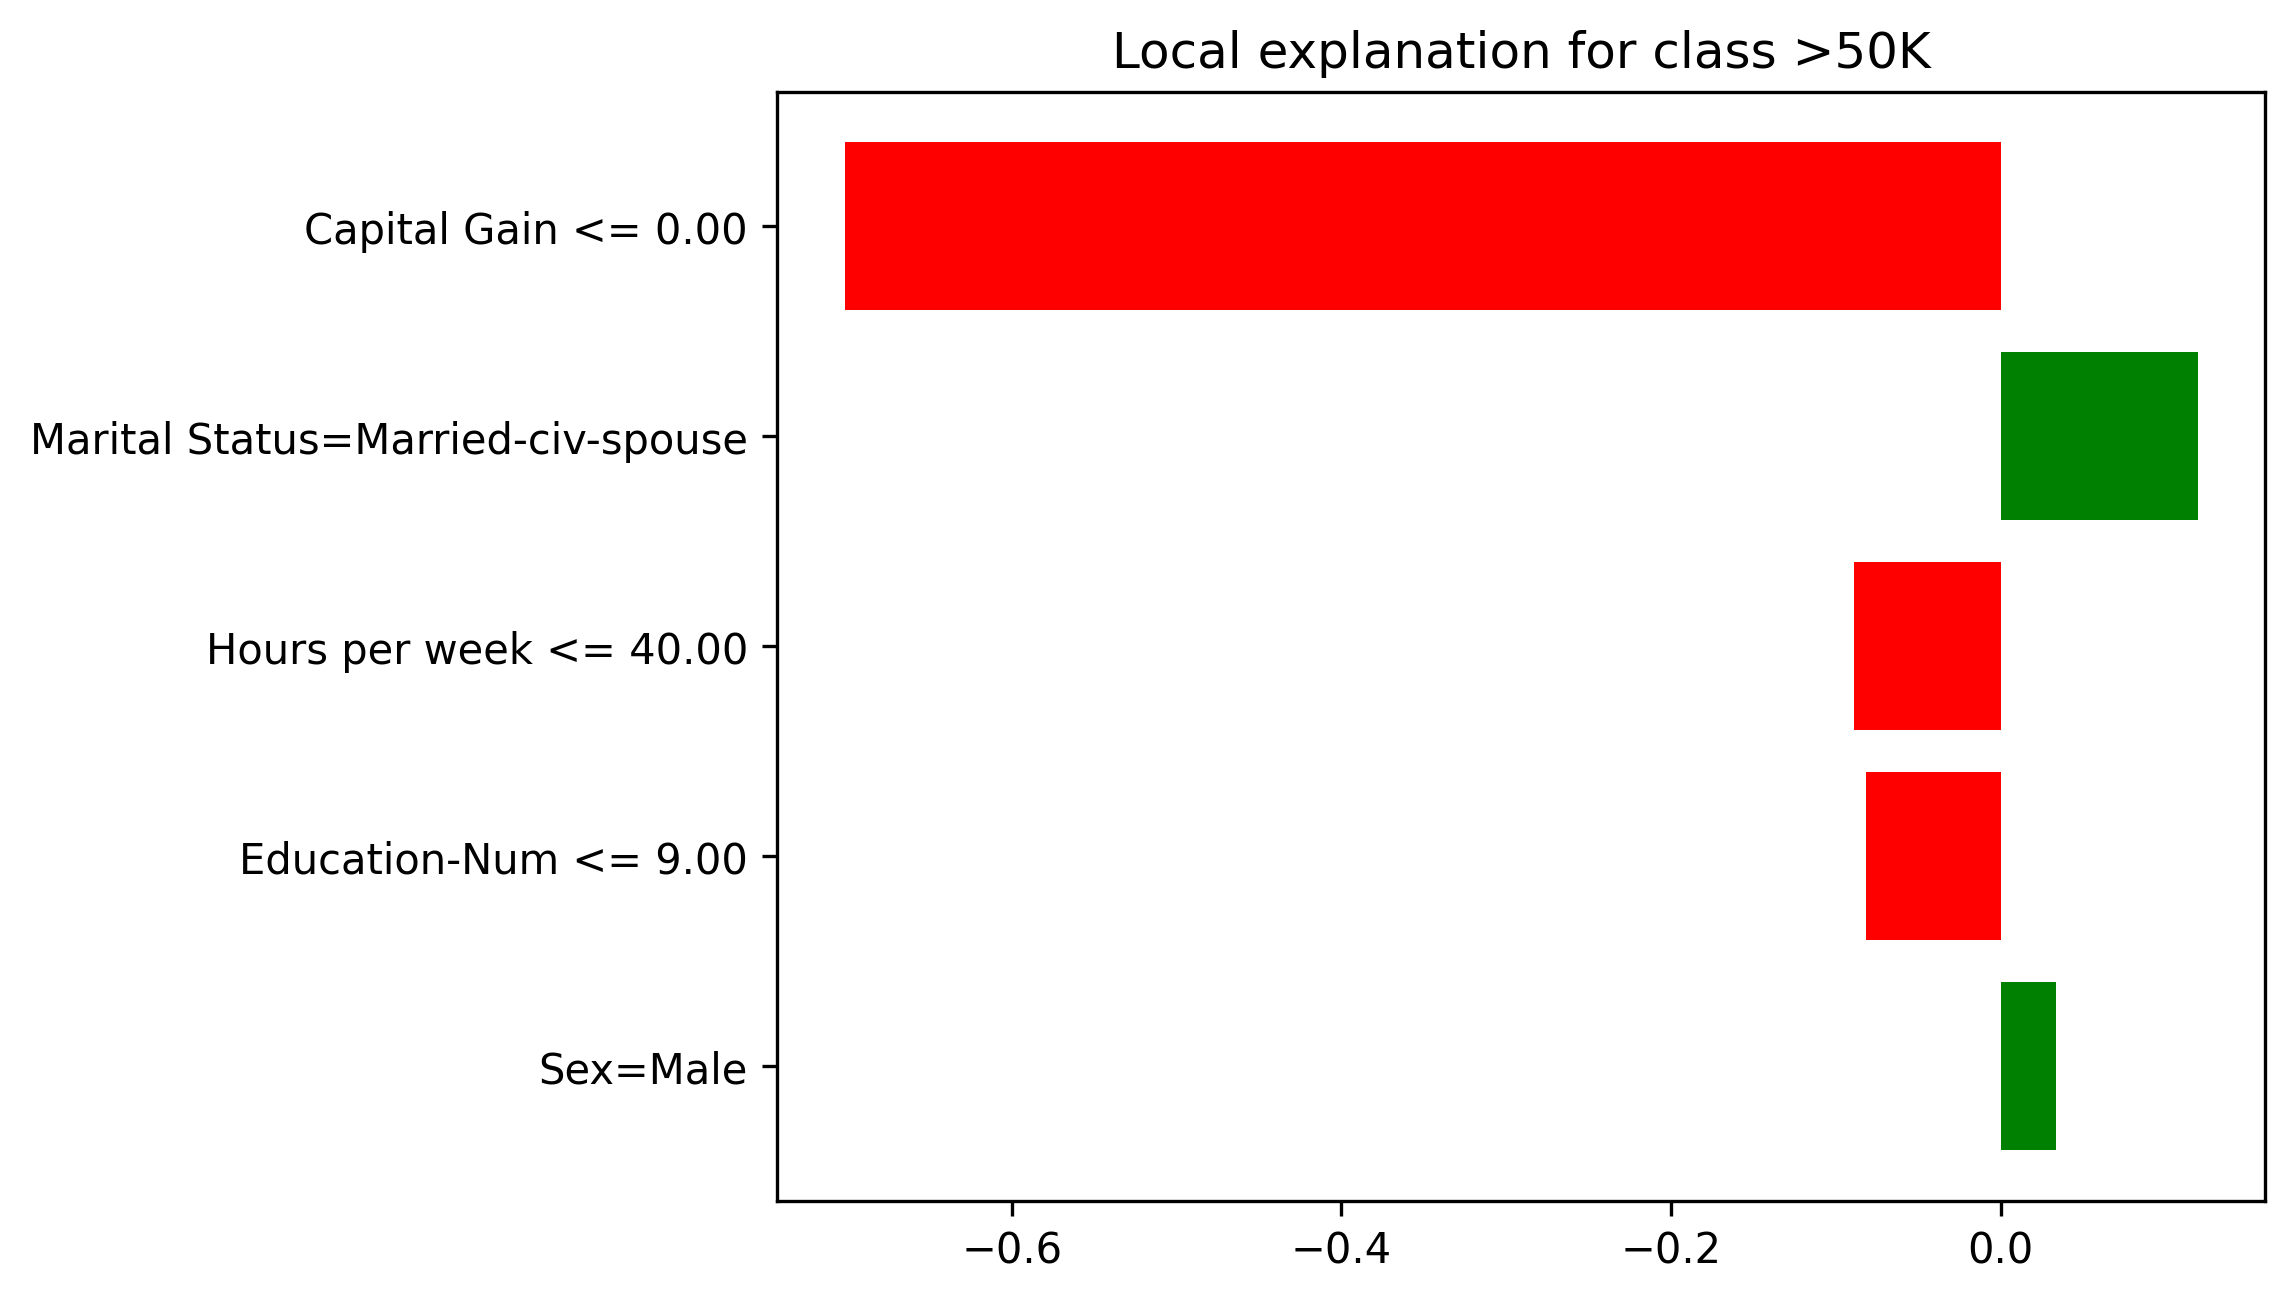
\includegraphics[width=\textwidth]{../out/xgboost-92.png}
    \caption{XGBoost}
  \end{subfigure}
  \caption{Wyjaśnienia LIME dla przykładu 92}
\end{figure}

\subsubsection{Przykład 18}

Oba modele poprawnie przewidziały <=50K. Oba interpretowały Capital Gain jako pozytywny czynnik, ale MLP przypisał niższą wagę niż XGBoost. Czynnik Hours per week był negatywny dla obu modeli.

\begin{figure}[H]
  \centering
  \begin{subfigure}{0.45\textwidth}
    \centering
    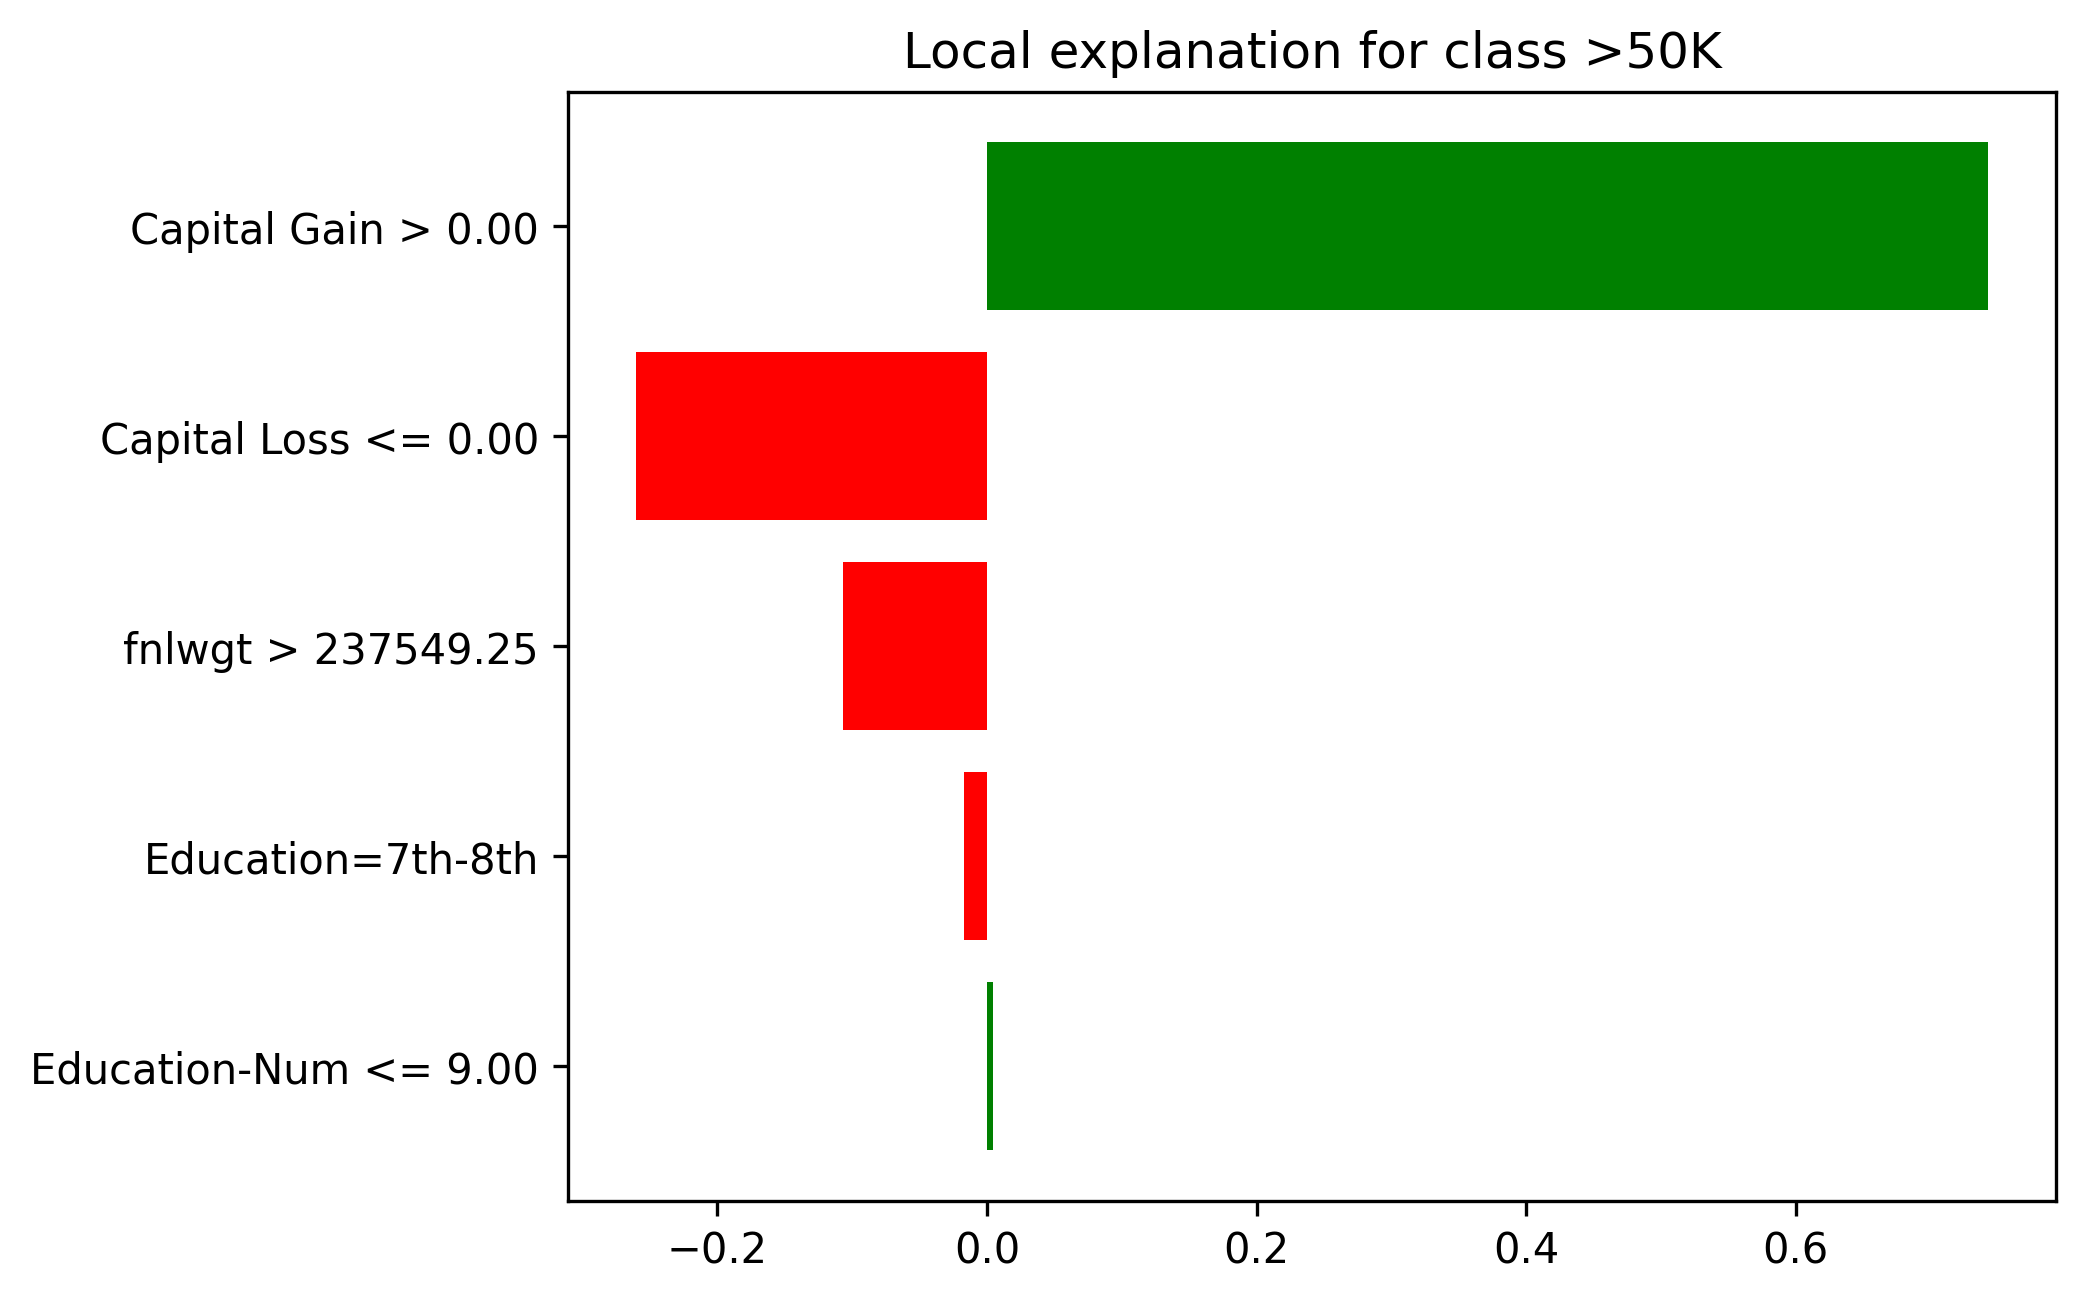
\includegraphics[width=\textwidth]{../out/mlp-18.png}
    \caption{MLPClassifier}
  \end{subfigure}
  \begin{subfigure}{0.45\textwidth}
    \centering
    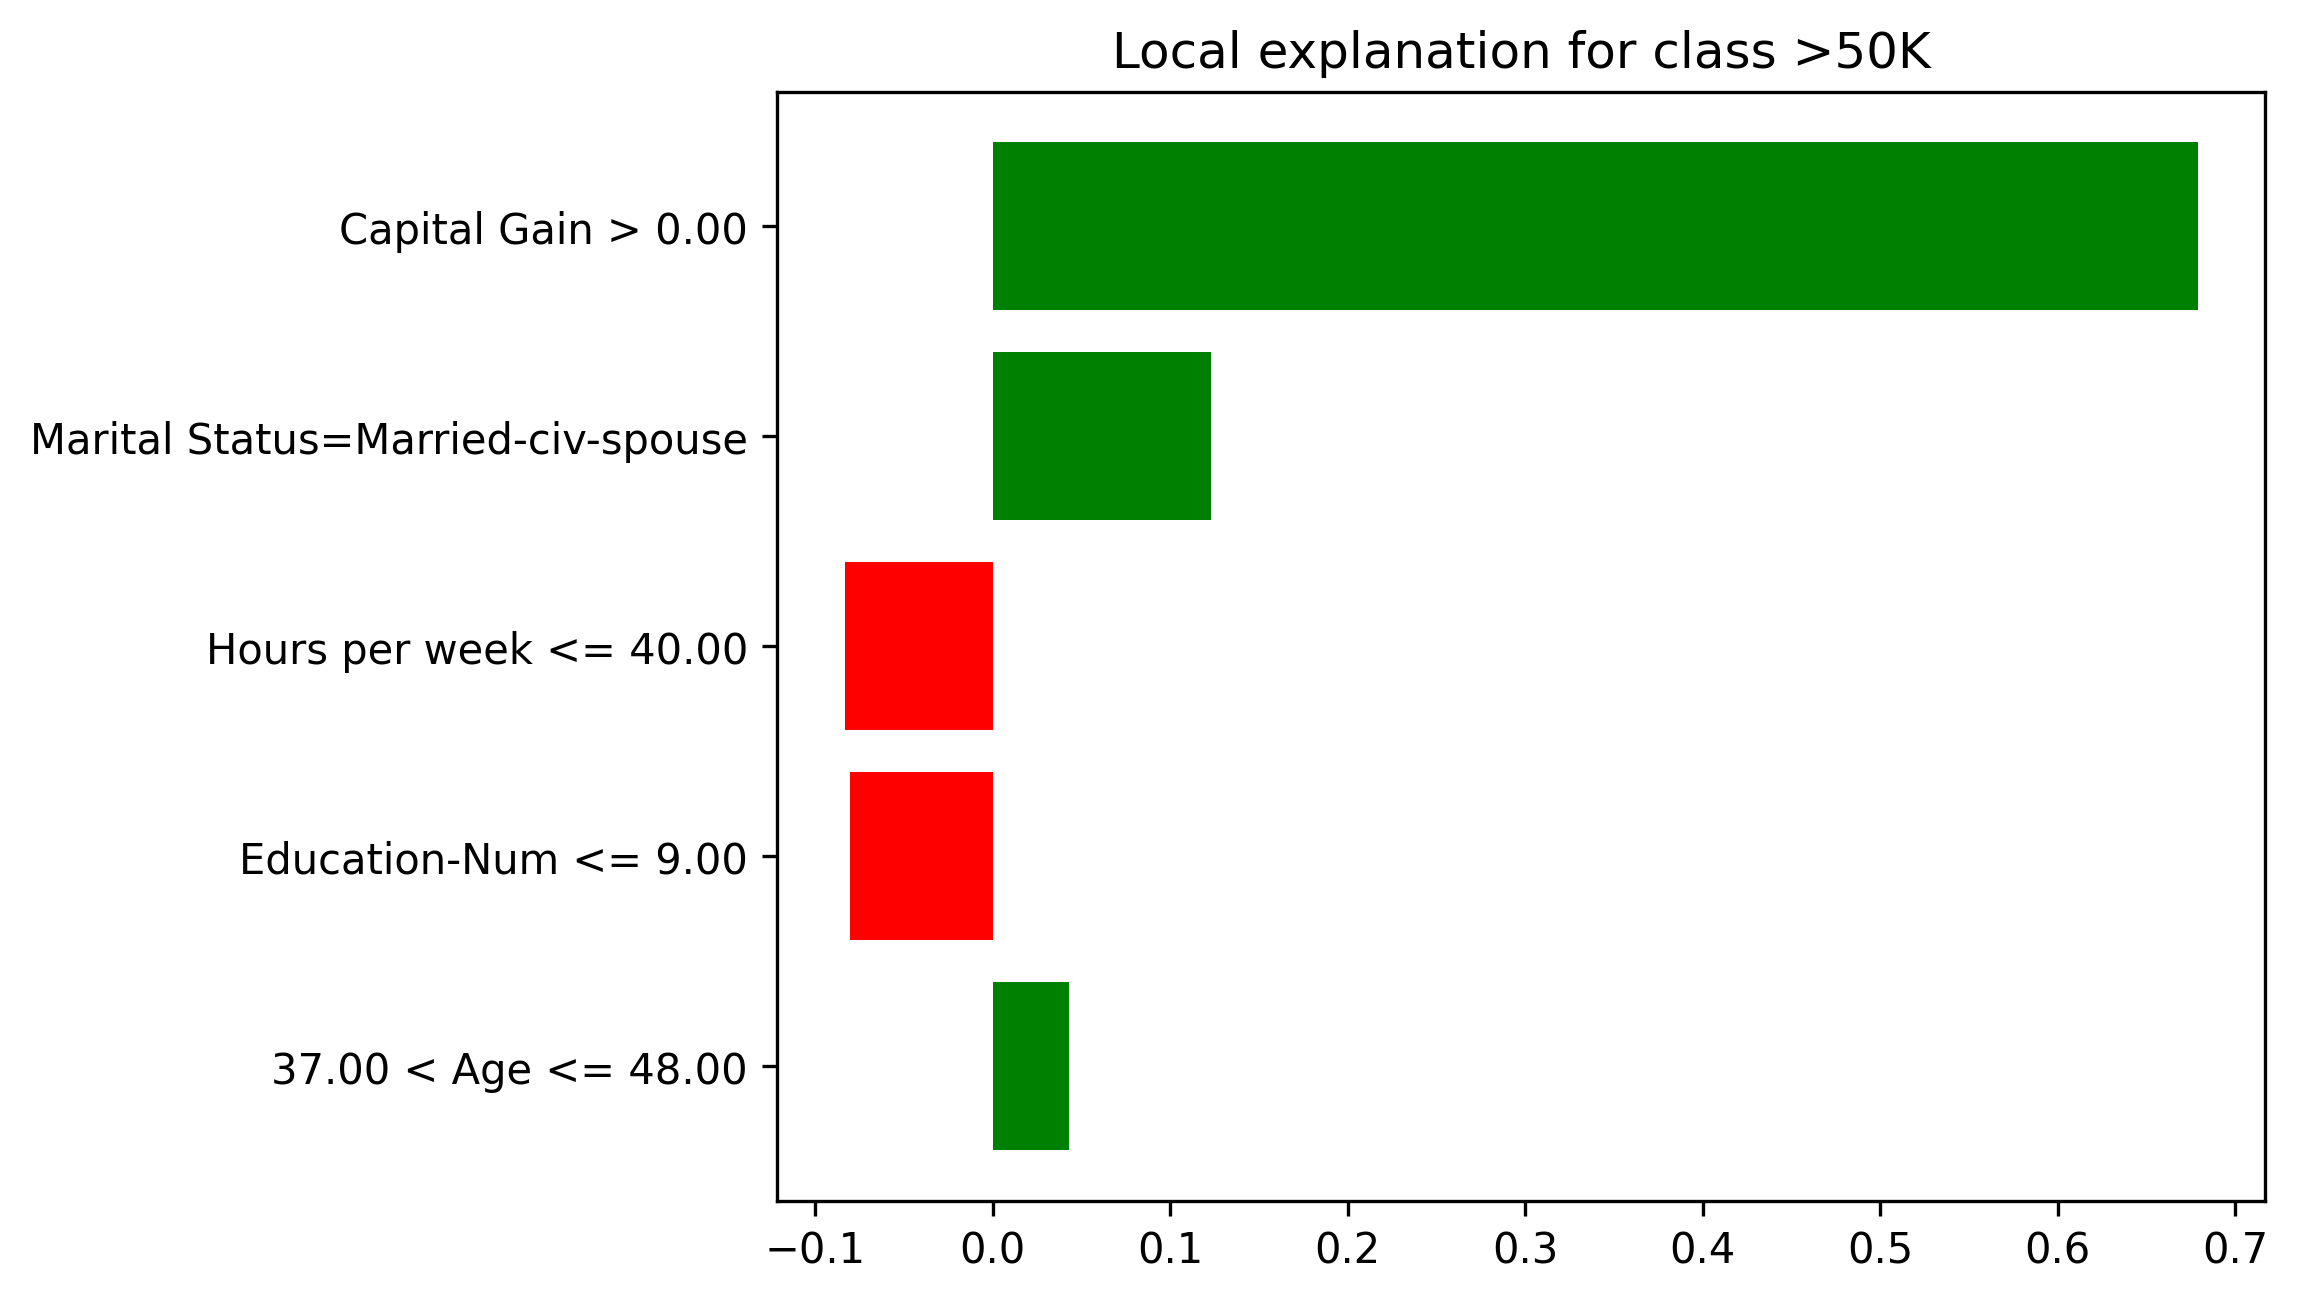
\includegraphics[width=\textwidth]{../out/xgboost-18.png}
    \caption{XGBoost}
  \end{subfigure}
  \caption{Wyjaśnienia LIME dla przykładu 18}
\end{figure}

\subsection{Analiza błędnej predykcji MLP}

Znaleziono przykład z błędną klasyfikacją MLP (etykieta: >50K, predykcja: <=50K, 85.1\% pewności). LIME ujawnił główne czynniki zmyłające model:

\begin{itemize}
  \item Capital Gain <= 0.00 (waga: -0.726) - brak zysków kapitałowych jako silny negatywny czynnik
  \item Capital Loss <= 0.00 (waga: -0.253) - brak strat kapitałowych jako negatywny czynnik
  \item fnlwgt w zakresie 117618-178587 (waga: +0.019) - minimalny pozytywny wpływ
  \item Sex=Male (waga: +0.007) - bardzo niska waga pozytywna
  \item Marital Status=Married-civ-spouse (waga: +0.007) - bardzo niska waga pozytywna
\end{itemize}

Model został zmyłony przez brak wskaźników kapitałowych, które przeważyły nad innymi czynnikami dochodowymi. LIME pokazuje, że model lokalnie przewiduje 15.4\% prawdopodobieństwa dla >50K, ale globalna predykcja MLP wynosi 14.9\%.

\begin{figure}[H]
  \centering
  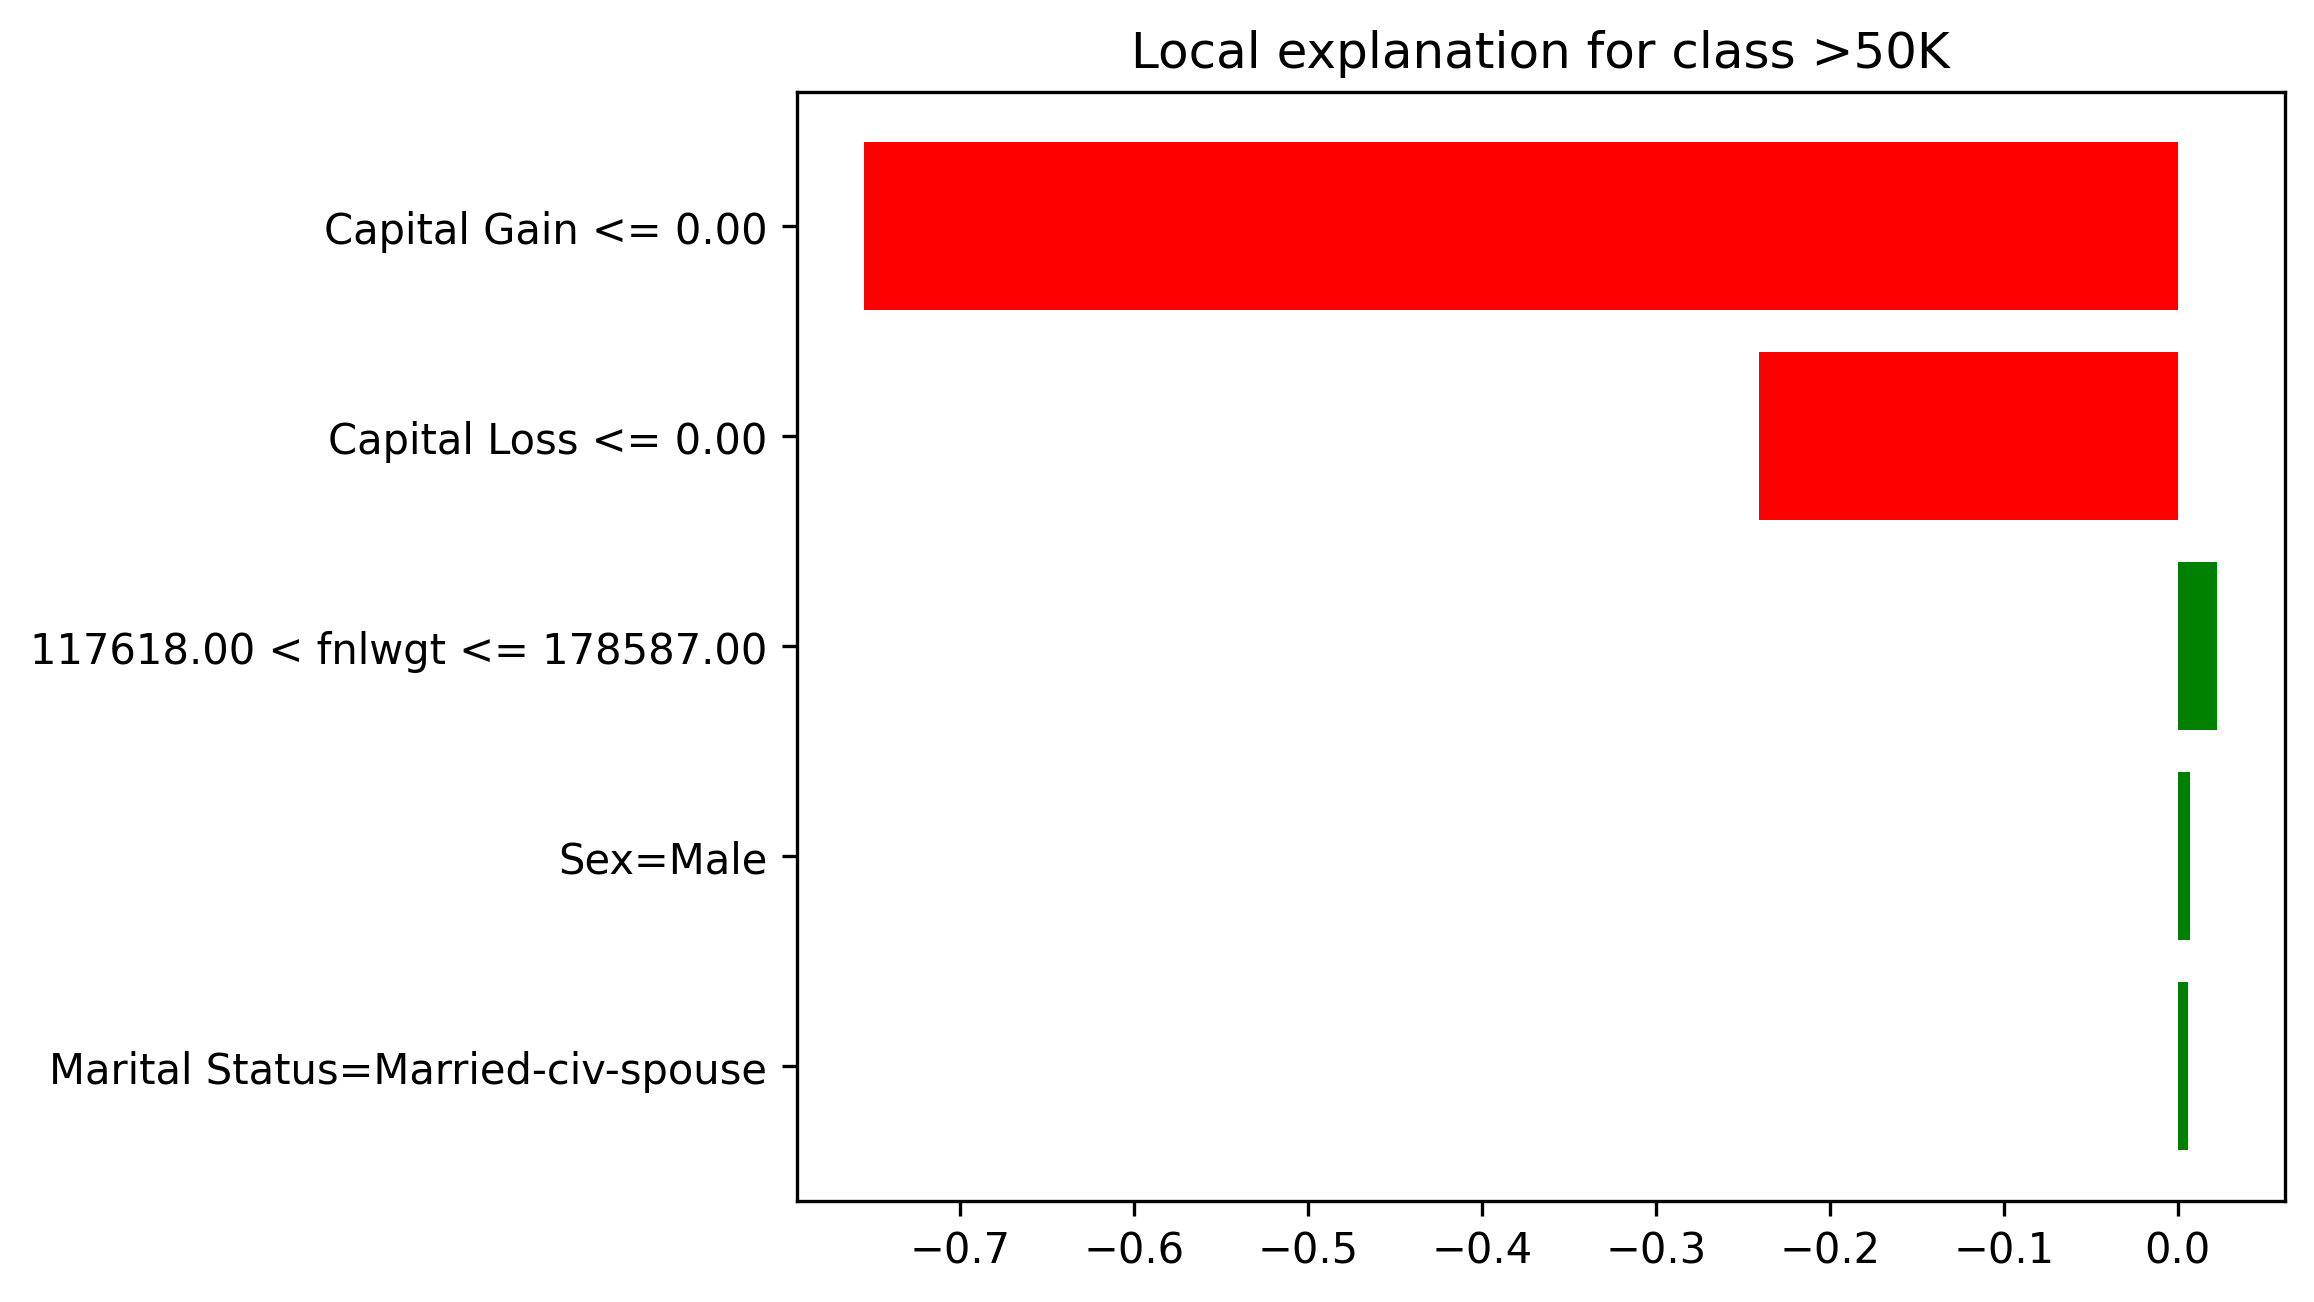
\includegraphics[width=0.6\textwidth]{../out/mlp-wrong.png}
  \caption{Wyjaśnienia LIME dla błędnej predykcji MLP}
\end{figure}

\subsection{Interesujący przypadek}

Przeanalizowano osobę z wysokim wykształceniem (Education-Num > 12) ale niskim dochodem (<=50K). Ten przypadek jest interesujący, ponieważ wykształcenie powinno korelować z dochodem, ale tutaj osoba z wysokim wykształceniem ma niski dochód. MLP poprawnie przewidział <=50K, pokazując, że inne czynniki (wiek, zawód, Capital Gain/Loss) przeważyły nad wykształceniem. LIME ujawnił, że model rozpoznał inne czynniki jako ważniejsze niż samo wykształcenie.

\begin{figure}[H]
  \centering
  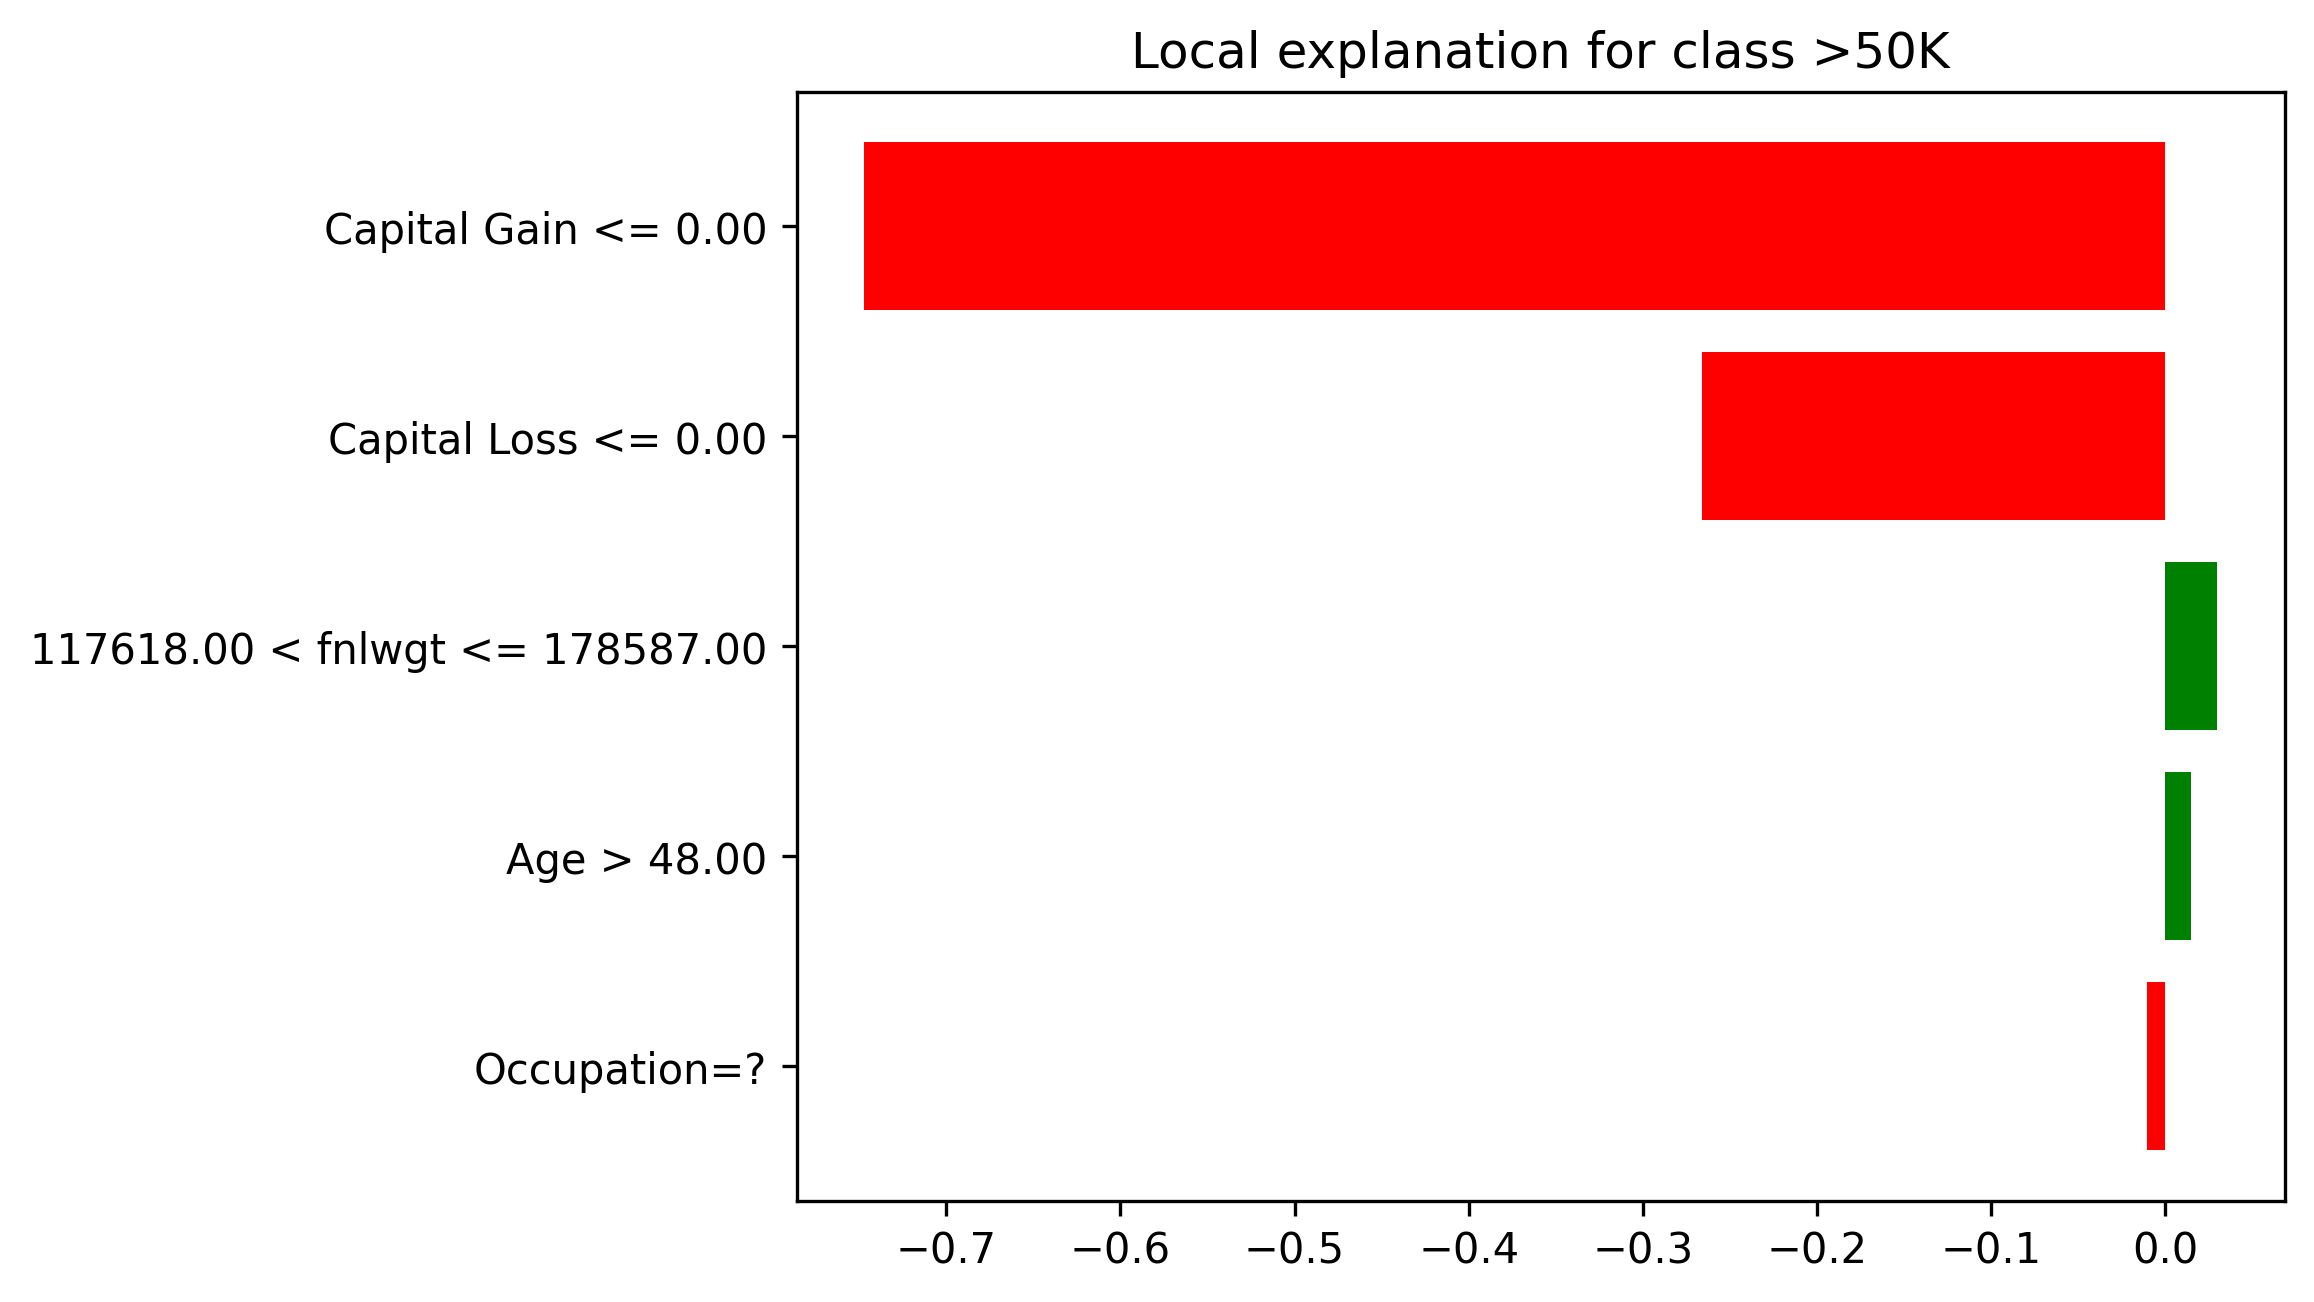
\includegraphics[width=0.6\textwidth]{../out/mlp-interesting.png}
  \caption{Wyjaśnienia LIME dla interesującego przypadku}
\end{figure}

\section{Analiza obrazów - LIME}

\subsection{Wybór obrazu}

Wybrano obraz smartfona z klawiaturą (smartphone.jpg) spoza zbioru ImageNet. Obraz przedstawia telefon komórkowy leżący obok fragmentu klawiatury komputerowej na drewnianym blacie.

\begin{figure}[H]
  \centering
  
\includegraphics[width=0.6\textwidth]{../data/smartphone.jpg}
  \caption{Oryginalny obraz smartfona z klawiaturą}
\end{figure}

\subsection{Analiza z wykorzystaniem różnych sieci}

Wykorzystano dwie sieci neuronowe: ResNet50 i VGG16.

\textbf{ResNet50:}
\begin{itemize}
  \item Najbardziej prawdopodobna klasa: cellular\_telephone (57.8\%) - telefon komórkowy
  \item Pozostałe klasy: iPod (20.7\%), notebook (9.8\%), remote\_control (4.1\%)
\end{itemize}

\textbf{VGG16:}
\begin{itemize}
  \item Najbardziej prawdopodobna klasa: iPod (75.8\%) - odtwarzacz iPod
  \item Pozostałe klasy: cellular\_telephone (13.1\%), notebook (5.8\%), space\_bar (1.1\%)
\end{itemize}

\begin{figure}[H]
  \centering
  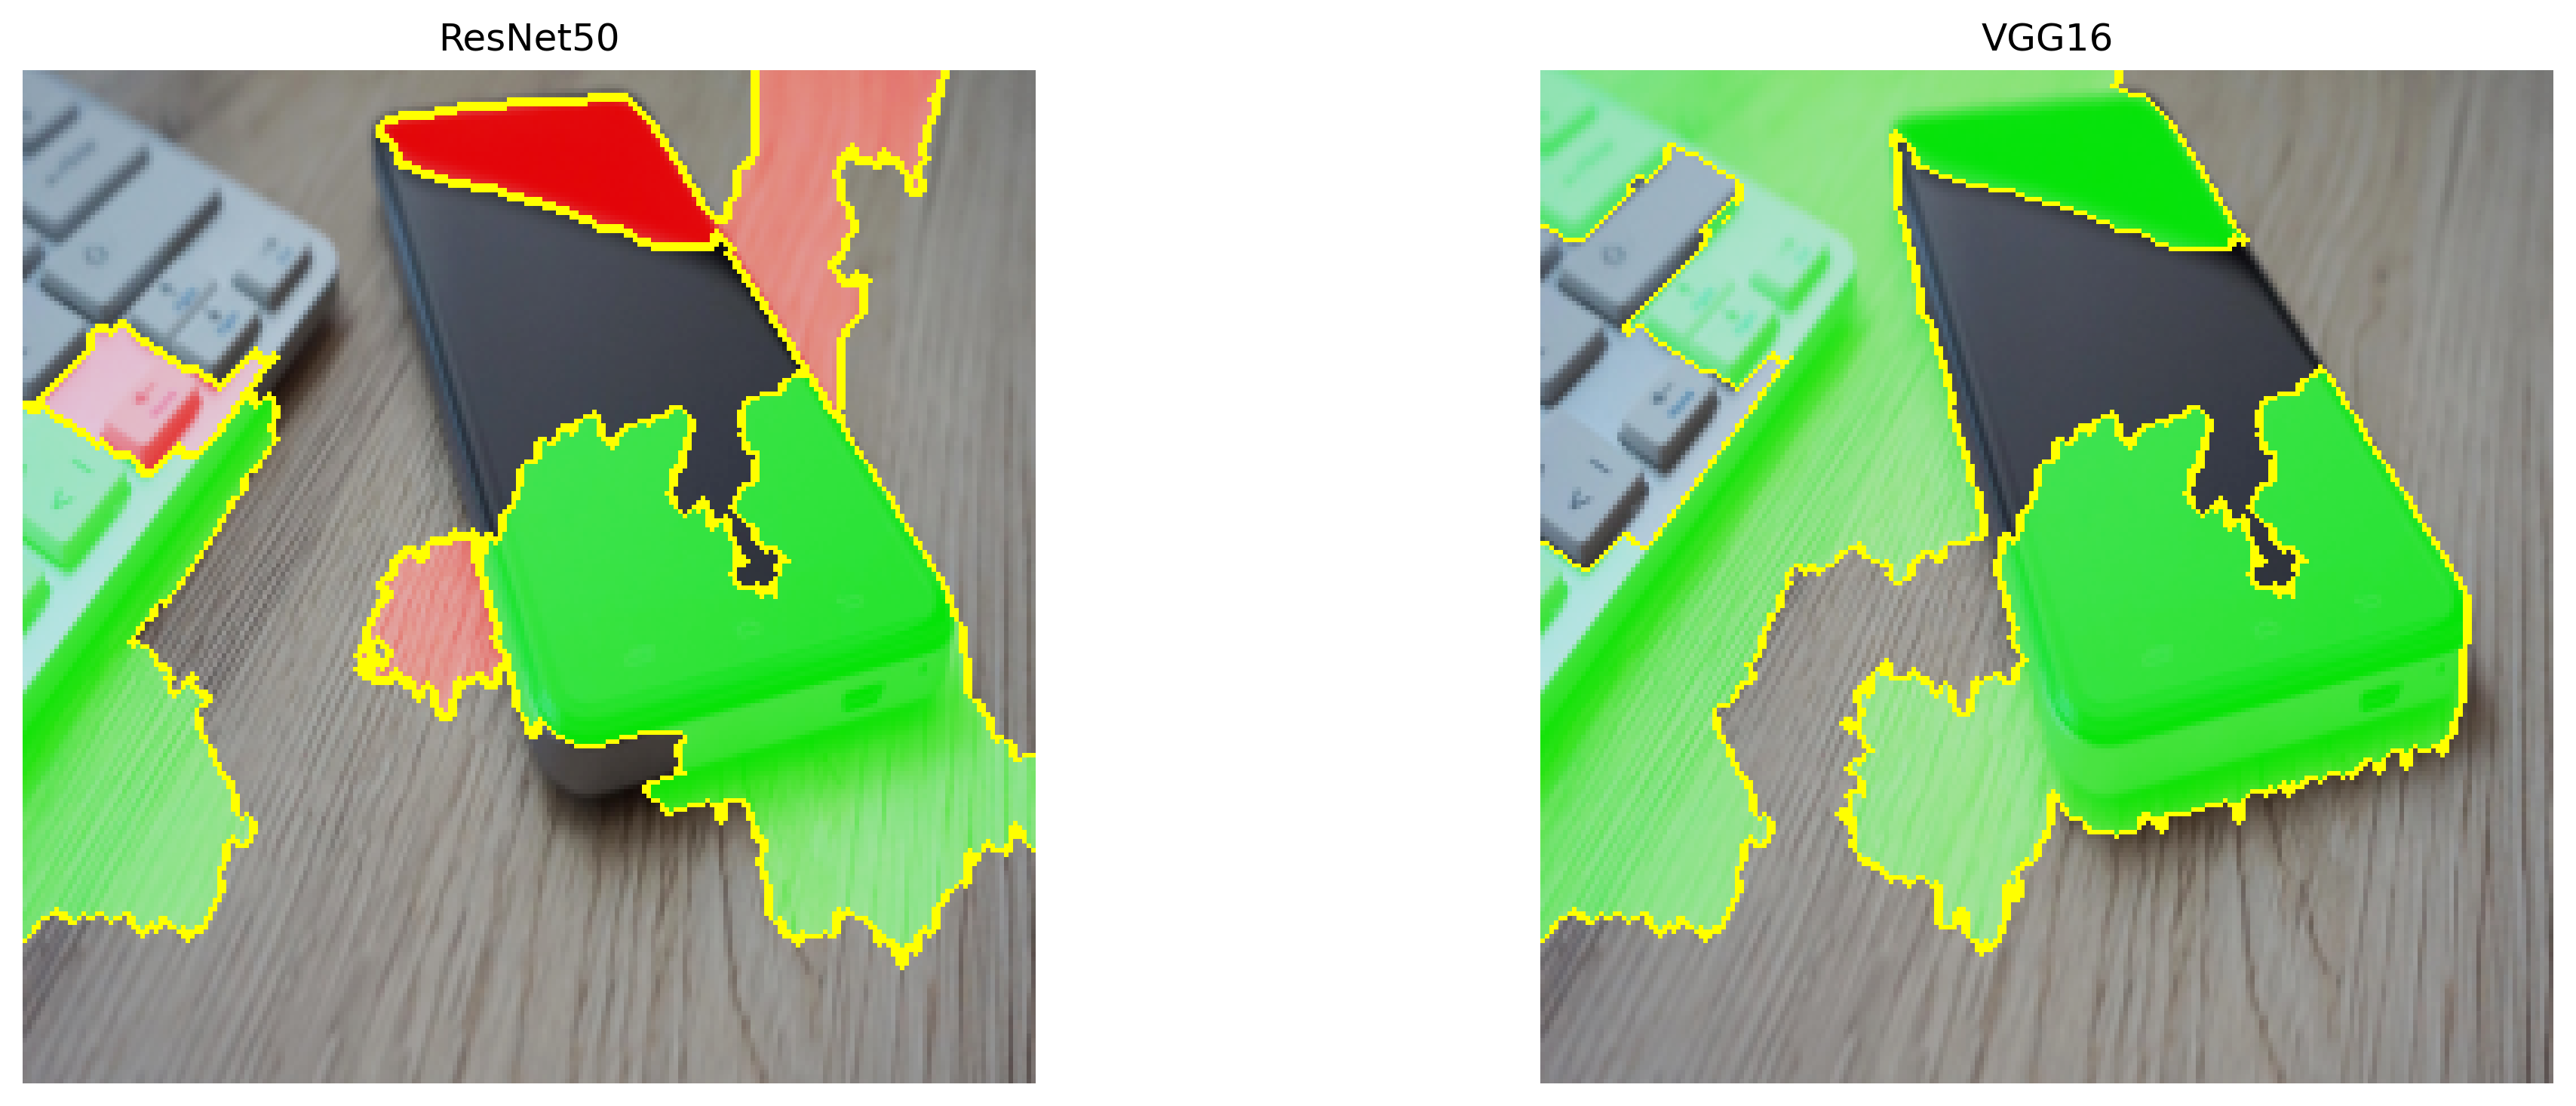
\includegraphics[width=0.8\textwidth]{../out/ResNet50vsVGG16.png}
  \caption{Porównanie wyjaśnień LIME dla ResNet50 i VGG16}
\end{figure}

\subsection{Analiza po usunięciu kluczowych cech}

Po usunięciu najważniejszych superpikseli (negative\_only=True):

\textbf{ResNet50:}
\begin{itemize}
  \item Nowa najbardziej prawdopodobna klasa: pencil\_sharpener (96.0\%) - ostrzałka
\end{itemize}

\textbf{VGG16:}
\begin{itemize}
  \item Nowa najbardziej prawdopodobna klasa: space\_shuttle (33.2\%) - statek kosmiczny
  \item Druga najbardziej prawdopodobna klasa: syringe (13.8\%) - strzykawka
\end{itemize}

\begin{figure}[H]
  \centering
  \begin{subfigure}{0.45\textwidth}
    \centering
    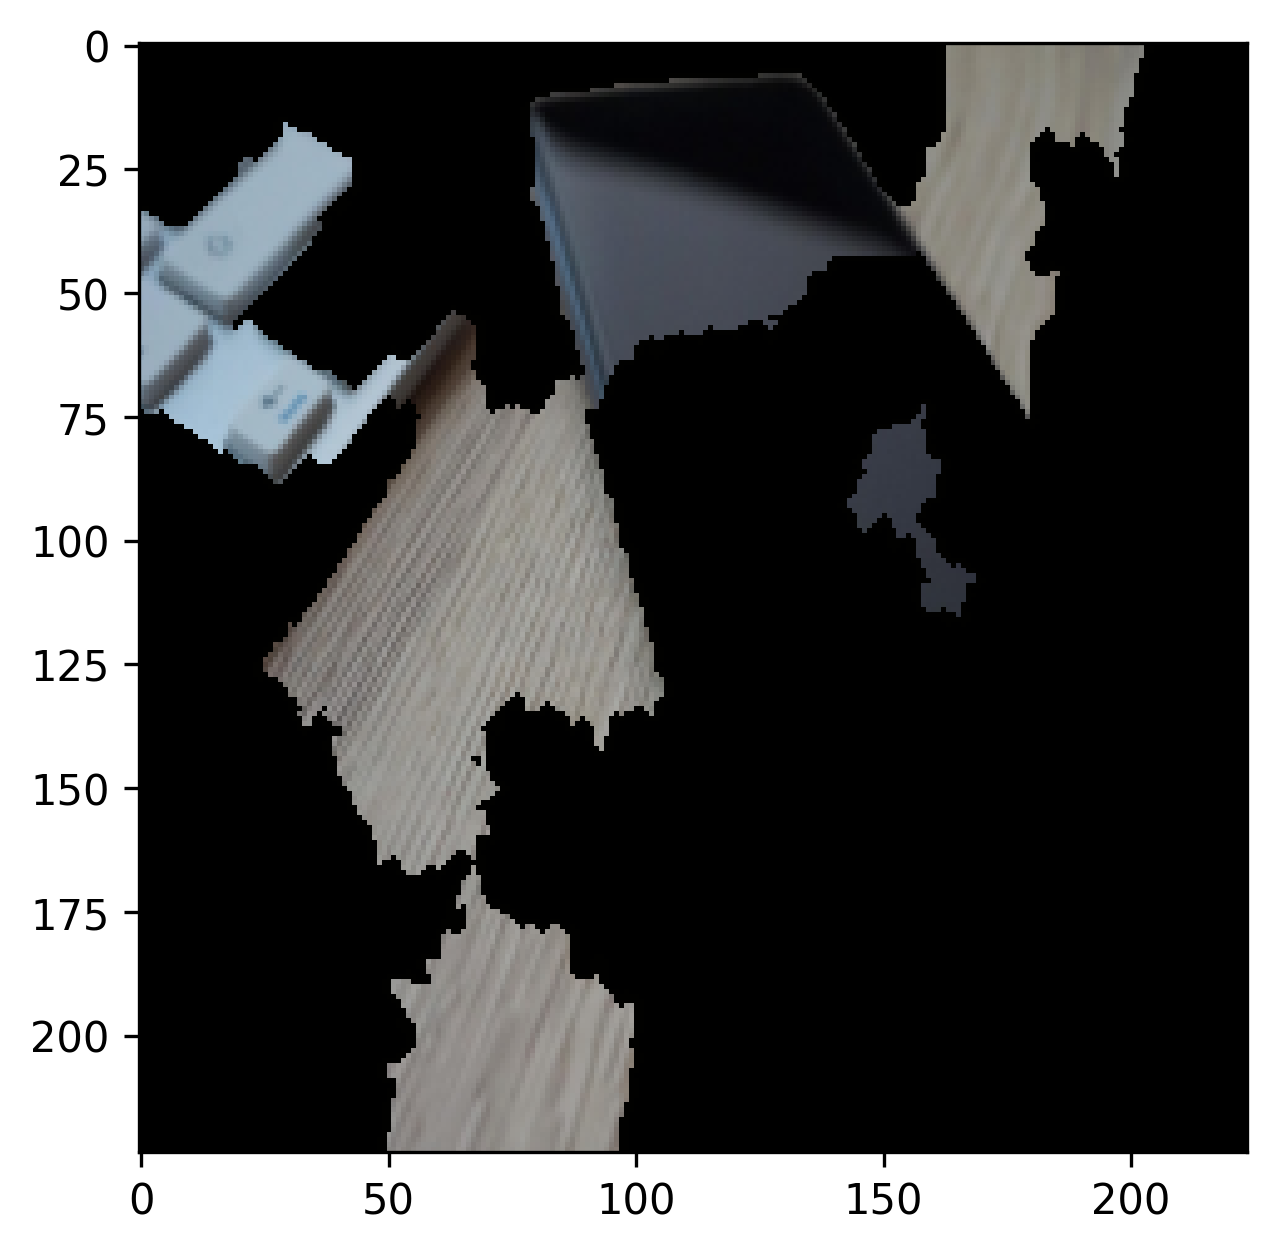
\includegraphics[width=\textwidth]{../out/ResNet50-hidden.png}
    \caption{ResNet50 - bez kluczowych cech}
  \end{subfigure}
  \begin{subfigure}{0.45\textwidth}
    \centering
    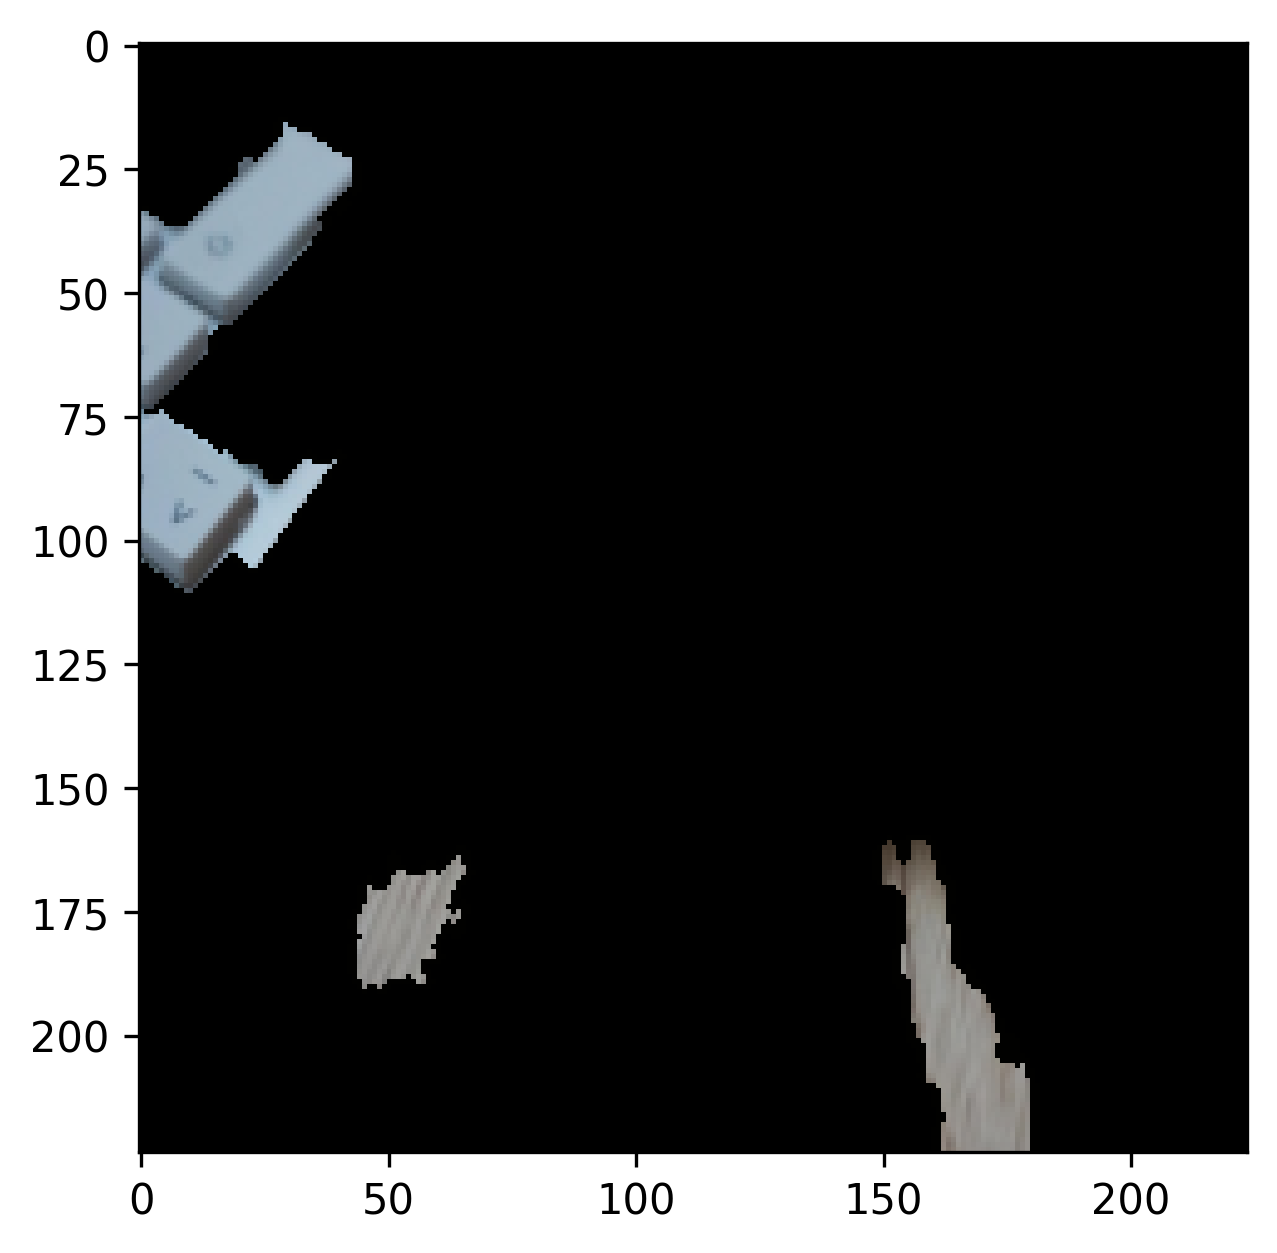
\includegraphics[width=\textwidth]{../out/VGG16-hidden.png}
    \caption{VGG16 - bez kluczowych cech}
  \end{subfigure}
\end{figure}

\begin{figure}[H]
  \centering
  \begin{subfigure}{0.45\textwidth}
    \centering
    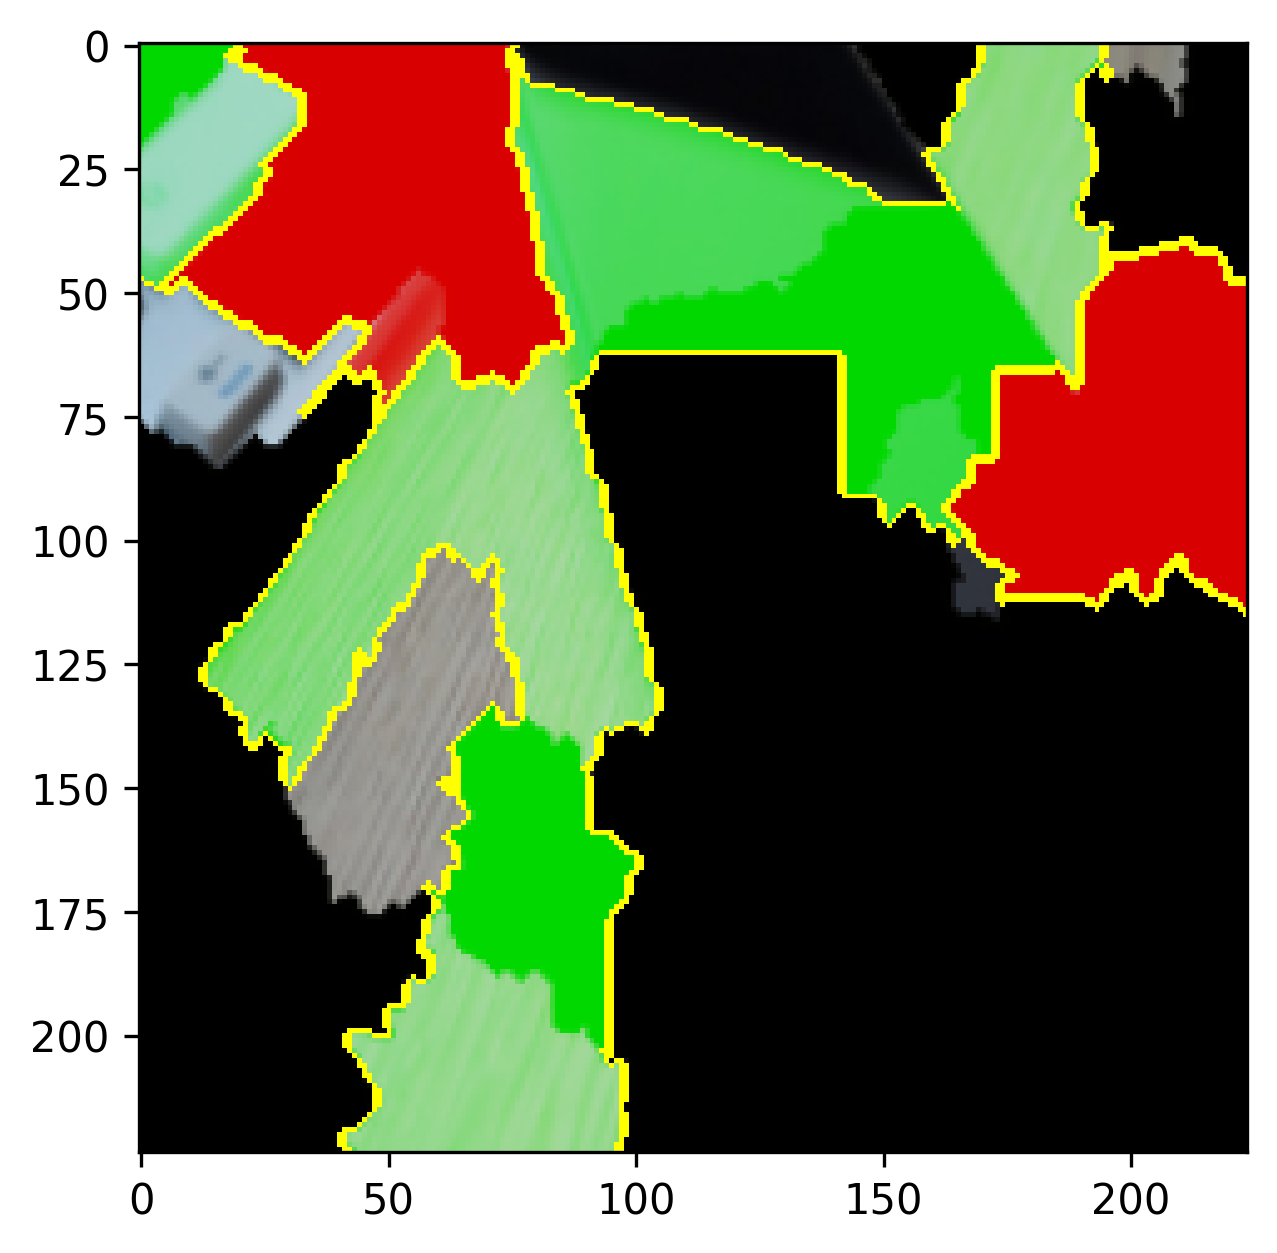
\includegraphics[width=\textwidth]{../out/ResNet50-hidden-explained.png}
    \caption{ResNet50 - z wyjaśnieniem}
  \end{subfigure}
  \begin{subfigure}{0.45\textwidth}
    \centering
    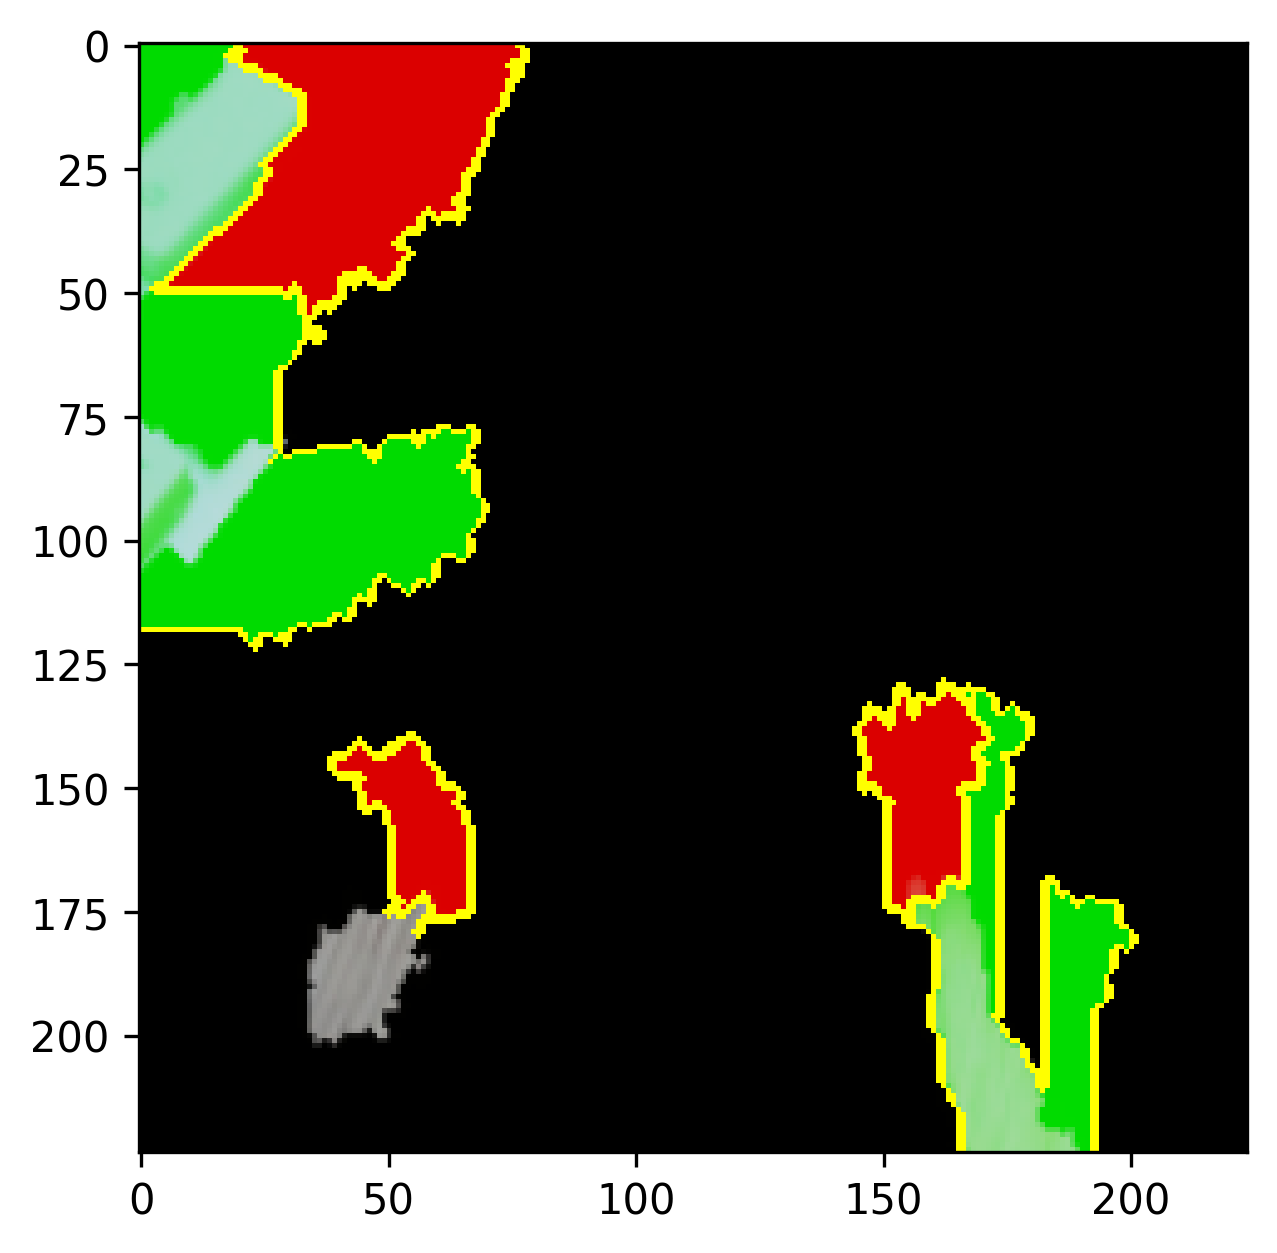
\includegraphics[width=\textwidth]{../out/VGG16-hidden-explained.png}
    \caption{VGG16 - z wyjaśnieniem}
  \end{subfigure}
\end{figure}

\section{Wnioski}

LIME skutecznie identyfikuje kluczowe cechy wpływające na predykcje (Capital Gain/Loss, wykształcenie, wiek), ale jest to tylko lokalna aproksymacja modelu. LIME może popełniać błędy i nie zawsze dokładnie odzwierciedla globalne zachowanie modelu - pokazuje przybliżoną ważność cech wybranych przez rzeczywisty model. Porównanie MLP z XGBoost wykazało różne wzorce interpretowalności, co pokazuje, że LIME ujawnia różnice w sposobie uczenia się modeli.

W analizie obrazów, LIME skutecznie identyfikował kluczowe regiony, ale różne sieci (ResNet50 vs VGG16) interpretowały te same regiony inaczej. Usunięcie kluczowych cech prowadziło do drastycznej zmiany klasyfikacji.

\end{document}
